\section{Methodology}
\label{sec:methodology}

In this section, we present the architecture and mathematical formulation of the \textbf{Vision-Geometry-Action (VGA)} framework. An overview of the end-to-end policy pipeline is illustrated in Fig.~\ref{fig:architecture}.

\begin{figure*}[!t]
\centering
\IfFileExists{figures/vga_architecture.pdf}{%
    \includegraphics[width=0.92\textwidth]{figures/vga_architecture.pdf}%
}{%
    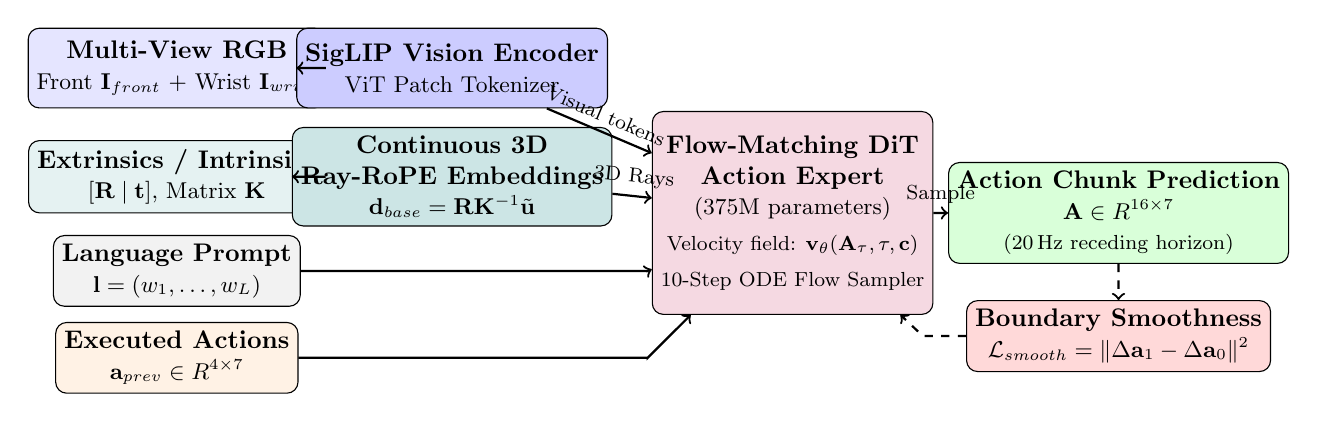
\begin{tikzpicture}[scale=0.92, every node/.style={transform shape}]
        % Input blocks
        \node[draw, fill=blue!10, rounded corners, minimum width=2.6cm, minimum height=1.1cm, align=center] (obs) at (0, 2.2) {\textbf{Multi-View RGB}\\\small Front $\mathbf{I}_{\text{front}}$ + Wrist $\mathbf{I}_{\text{wrist}}$};
        \node[draw, fill=teal!10, rounded corners, minimum width=2.6cm, minimum height=0.9cm, align=center] (geom) at (0, 0.7) {\textbf{Extrinsics / Intrinsics}\\\small $[\mathbf{R} \mid \mathbf{t}]$, Matrix $\mathbf{K}$};
        \node[draw, fill=gray!10, rounded corners, minimum width=2.6cm, minimum height=0.8cm, align=center] (lang) at (0, -0.6) {\textbf{Language Prompt}\\\small $\mathbf{l} = (w_1, \dots, w_L)$};
        \node[draw, fill=orange!10, rounded corners, minimum width=2.6cm, minimum height=0.8cm, align=center] (prev) at (0, -1.8) {\textbf{Executed Actions}\\\small $\mathbf{a}_{\text{prev}} \in \mathbb{R}^{4 \times 7}$};

        % Encoders
        \node[draw, fill=blue!20, rounded corners, minimum width=2.8cm, minimum height=1.1cm, align=center] (siglip) at (3.8, 2.2) {\textbf{SigLIP Vision Encoder}\\\small ViT Patch Tokenizer};
        \node[draw, fill=teal!20, rounded corners, minimum width=3.0cm, minimum height=1.1cm, align=center] (rayrope) at (3.8, 0.7) {\textbf{Continuous 3D}\\\textbf{Ray-RoPE Embeddings}\\\small $\mathbf{d}_{\text{base}} = \mathbf{R} \mathbf{K}^{-1} \tilde{\mathbf{u}}$};

        % Fusion / Conditioning
        \node[draw, fill=purple!15, rounded corners, minimum width=3.3cm, minimum height=2.8cm, align=center] (dit) at (8.5, 0.2) {\textbf{Flow-Matching DiT}\\\textbf{Action Expert}\\\small (375M parameters)\\[2pt]\footnotesize Velocity field: $\mathbf{v}_\theta(\mathbf{A}_\tau, \tau, \mathbf{c})$\\[2pt]\footnotesize 10-Step ODE Flow Sampler};

        % Output chunk and smoothing
        \node[draw, fill=green!15, rounded corners, minimum width=2.8cm, minimum height=1.3cm, align=center] (chunk) at (13.0, 0.2) {\textbf{Action Chunk Prediction}\\\small $\mathbf{A} \in \mathbb{R}^{16 \times 7}$\\\footnotesize (20\,Hz receding horizon)};
        \node[draw, fill=red!15, rounded corners, minimum width=2.8cm, minimum height=0.9cm, align=center] (smooth) at (13.0, -1.5) {\textbf{Boundary Smoothness}\\\small $\mathcal{L}_{\text{smooth}} = \|\Delta \mathbf{a}_1 - \Delta \mathbf{a}_0\|^2$};

        % Connectors
        \draw[->, thick] (obs) -- (siglip);
        \draw[->, thick] (geom) -- (rayrope);
        \draw[->, thick] (siglip) -- (dit) node[midway, above, sloped] {\footnotesize Visual tokens};
        \draw[->, thick] (rayrope) -- (dit) node[midway, above, sloped] {\footnotesize 3D Rays};
        \draw[->, thick] (lang) -| (6.5, -0.6) -- (dit);
        \draw[->, thick] (prev) -| (6.5, -1.8) -- (dit);
        \draw[->, thick] (dit) -- (chunk) node[midway, above] {\footnotesize Sample};
        \draw[->, dashed, thick] (chunk) -- (smooth);
        \draw[->, dashed, thick] (smooth) -| (10.3, -1.5) -- (dit);
    \end{tikzpicture}%
}
\caption{\textbf{Vision-Geometry-Action (VGA) Policy Architecture.} Multi-view camera observations (static front and dynamic wrist) are processed through a SigLIP vision backbone, where patch tokens are modulated by continuous 3D Ray-RoPE encoding metric optical ray vectors $\mathbf{d}_{\text{base}} = \mathbf{R}_{\text{base}\leftarrow\text{cam}} \mathbf{K}^{-1} \tilde{\mathbf{u}}$. A lightweight Flow-Matching Diffusion Transformer (DiT) action expert generates continuous 16-step 7-DoF action chunks conditioned on language goals and the prior executed action prefix $\mathbf{a}_{\text{prev}}$. An explicit chunk-boundary loss ($\mathcal{L}_{\text{smooth}}$) enforces $C^1$ velocity continuity, eliminating inter-chunk acceleration spikes.}
\label{fig:architecture}
\vspace{-2mm}
\end{figure*}

\subsection{Problem Formulation and Policy Interface}
We formulate language-conditioned robot manipulation as a continuous receding-horizon control problem. At control step $k$, the policy receives:
\begin{enumerate}
    \item Multi-view visual observations consisting of a static third-person camera image $\mathbf{I}_{\text{front}} \in \mathbb{R}^{H_v \times W_v \times 3}$ and an eye-in-hand wrist camera image $\mathbf{I}_{\text{wrist}} \in \mathbb{R}^{H_v \times W_v \times 3}$.
    \item Known camera intrinsic matrices $\mathbf{K} \in \mathbb{R}^{3 \times 3}$ and extrinsic transformation matrices $\mathbf{T}_{\text{base}\leftarrow\text{cam}} = [\mathbf{R} \mid \mathbf{t}] \in \text{SE}(3)$ relating camera optical frames to the physical robot base.
    \item A natural language task prompt $\mathbf{l} = (w_1, \dots, w_L)$.
    \item A history prefix of the $P$ most recently executed physical actions $\mathbf{a}_{\text{prev}} \in \mathbb{R}^{P \times D_a}$ ($P=4, D_a=7$).
\end{enumerate}

The policy predicts a continuous chunk of $H$ future end-effector actions:
\begin{equation}
\mathbf{A}_{k:k+H} = [\mathbf{a}_k, \mathbf{a}_{k+1}, \dots, \mathbf{a}_{k+H-1}] \in \mathbb{R}^{H \times D_a},
\end{equation}
where each action vector $\mathbf{a}_t = [\Delta x, \Delta y, \Delta z, \Delta \phi_x, \Delta \phi_y, \Delta \phi_z, g]^T$ comprises relative 3D Cartesian position deltas, 3D Euler orientation deltas in the robot base coordinate frame, and a binary gripper state $g \in \{0, 1\}$. In our canonical implementation, $H=16$ steps at a 20\,Hz control loop ($\Delta t = 0.05$\,s), corresponding to an 800\,ms physical predictive horizon.

\subsection{Continuous 3D Ray-RoPE Geometric Grounding}
Standard transformer backbones divide an image $\mathbf{I}$ into a grid of $M = (H_v/p) \times (W_v/p)$ patches and add 2D planar positional embeddings, blinding the model to 3D camera geometry. When camera extrinsics change, identical 2D pixel coordinates correspond to entirely different 3D physical workspace positions.

To overcome this without requiring active depth sensors or compute-heavy 3D point cloud convolutions, we introduce \textbf{Continuous 3D Ray-RoPE}. For each visual patch with center pixel coordinate $\mathbf{u} = (u, v)$ in the normalized image plane, we construct the homogeneous coordinate $\tilde{\mathbf{u}} = [u, v, 1]^T$. Using the camera intrinsic matrix $\mathbf{K}$, the optical ray vector in the camera frame is:
\begin{equation}
\mathbf{d}_{\text{cam}} = \mathbf{K}^{-1} \tilde{\mathbf{u}}, \quad \hat{\mathbf{d}}_{\text{cam}} = \frac{\mathbf{d}_{\text{cam}}}{\|\mathbf{d}_{\text{cam}}\|_2}.
\end{equation}
We then project this optical ray into the robot's base coordinate frame using the known extrinsic rotation $\mathbf{R}_{\text{base}\leftarrow\text{cam}}$:
\begin{equation}
\mathbf{d}_{\text{base}} = \mathbf{R}_{\text{base}\leftarrow\text{cam}} \hat{\mathbf{d}}_{\text{cam}} = [d_x, d_y, d_z]^T \in \mathbb{S}^2.
\end{equation}

For each attention query $\mathbf{q}_i$ and key $\mathbf{k}_j$ associated with visual patch tokens, we apply a continuous rotary transformation modulated by the metric 3D ray direction:
\begin{equation}
\mathbf{q}_i^{(m)} = \mathbf{R}_{\text{RoPE}}\left(\mathbf{d}_{\text{base}, i}, \theta_m\right) \mathbf{q}_i^{(m)},
\end{equation}
where $\mathbf{R}_{\text{RoPE}}$ applies continuous 2D rotation blocks in the latent channel dimension scaled by frequency bands $\theta_m = 10000^{-2m/d}$. Consequently, inner-product attention scores explicitly satisfy:
\begin{equation}
\langle \mathbf{q}_i, \mathbf{k}_j \rangle = f\left(\mathbf{d}_{\text{base}, i} - \mathbf{d}_{\text{base}, j}, \mathbf{x}_i, \mathbf{x}_j\right),
\end{equation}
ensuring that attention weights depend directly on relative 3D angular and directional geometry in the physical robot workspace, rather than arbitrary 2D pixel indices. Under camera translations or rotations, the transformed base-frame rays $\mathbf{d}_{\text{base}}$ remain invariant, preserving spatial reasoning under camera shifts.

\subsection{Flow-Matching Diffusion Transformer Action Expert}
We employ Conditional Flow Matching (CFM) \cite{peebles2023scalable,black2024pi_0} to generate continuous action chunks. Let $p_0(\mathbf{A}) = \mathcal{N}(\mathbf{0}, \mathbf{I})$ denote a standard Gaussian prior distribution, and let $p_1(\mathbf{A})$ represent the target distribution of ground-truth demonstration action chunks. We define a probability path $p_t(\mathbf{A}_t)$ for flow time $\tau \in [0, 1]$ via linear interpolation:
\begin{equation}
\mathbf{A}_\tau = (1 - \tau)\mathbf{A}_0 + \tau \mathbf{A}_1, \quad \mathbf{A}_0 \sim p_0, \; \mathbf{A}_1 \sim p_1.
\end{equation}
The corresponding analytical target vector field is simply the constant velocity:
\begin{equation}
\mathbf{u}_\tau(\mathbf{A}_1 \mid \mathbf{A}_0) = \mathbf{A}_1 - \mathbf{A}_0.
\end{equation}

A lightweight Diffusion Transformer (DiT) network $\mathbf{v}_\theta(\mathbf{A}_\tau, \tau, \mathbf{c})$ parameterized by weights $\theta$ is trained to predict this velocity vector field conditioned on multimodal context $\mathbf{c} = \{\mathbf{E}_{\text{vis}}, \mathbf{E}_{\text{lang}}, \mathbf{a}_{\text{prev}}\}$. The conditional flow matching loss is:
\begin{equation}
\mathcal{L}_{\text{CFM}}(\theta) = \mathbb{E}_{\tau \sim \mathcal{U}[0, 1], \mathbf{A}_0 \sim p_0, \mathbf{A}_1 \sim p_1} \left\| \mathbf{v}_\theta(\mathbf{A}_\tau, \tau, \mathbf{c}) - (\mathbf{A}_1 - \mathbf{A}_0) \right\|_2^2.
\end{equation}

During inference, starting from Gaussian noise $\mathbf{A}_0 \sim \mathcal{N}(\mathbf{0}, \mathbf{I})$, the continuous action chunk $\mathbf{A}_1$ is integrated over $N_{\text{step}}$ numerical steps using an Euler or Midpoint ODE solver:
\begin{equation}
\mathbf{A}_{\tau + \Delta \tau} = \mathbf{A}_\tau + \Delta \tau \cdot \mathbf{v}_\theta\left(\mathbf{A}_\tau, \tau, \mathbf{c}\right), \quad \Delta \tau = \frac{1}{N_{\text{step}}}.
\end{equation}
In our implementation, setting $N_{\text{step}} = 10$ provides real-time chunk inference within 152\,ms on an edge NVIDIA T4 GPU while preserving high rollout fidelity.

\subsection{Smooth Chunk Boundary Coupling}
A notorious drawback of action-chunking policies is chunk-boundary discontinuity: because chunks $\mathbf{A}^{(k-1)}$ and $\mathbf{A}^{(k)}$ are sampled independently, the transition between the last action of chunk $k-1$ and the first action of chunk $k$ produces severe acceleration and jerk spikes.

To eliminate this boundary artifact, VGA incorporates two complementary mechanisms:
\begin{enumerate}
    \item \textbf{Receding Prior-Action Token Conditioning:} The action expert prepends the $P=4$ most recently executed physical actions $\mathbf{a}_{\text{prev}} = [\mathbf{a}_{-P+1}, \dots, \mathbf{a}_0]$ as fixed context tokens into the DiT attention sequence, anchoring the initial state and velocity.
    \item \textbf{Analytical Boundary Velocity Penalty ($\mathcal{L}_{\text{smooth}}$):} We enforce first-order velocity continuity ($C^1$) across the temporal boundary by regularizing velocity mismatch between the prior chunk tail and newly predicted chunk head:
    \begin{equation}
    \mathcal{L}_{\text{smooth}} = \left\| (\mathbf{a}_1 - \mathbf{a}_0) - (\mathbf{a}_0 - \mathbf{a}_{-1}) \right\|_2^2,
    \end{equation}
    where $\mathbf{a}_{-1}, \mathbf{a}_0$ denote the two most recent executed physical steps, and $\mathbf{a}_1$ is the first predicted action step of the new chunk.
\end{enumerate}

Binary gripper activation is trained using a transition-weighted binary cross-entropy loss:
\begin{equation}
\mathcal{L}_{\text{grip}} = -\sum_{t=1}^H w_t \left[ g_t \log \hat{g}_t + (1 - g_t) \log (1 - \hat{g}_t) \right],
\end{equation}
preventing intermediate floating-point gripper drift.

The overall training objective is optimized end-to-end:
\begin{equation}
\mathcal{L}_{\text{total}} = \mathcal{L}_{\text{CFM}} + \lambda_{\text{smooth}} \mathcal{L}_{\text{smooth}} + \lambda_{\text{grip}} \mathcal{L}_{\text{grip}},
\end{equation}
with default balancing weights $\lambda_{\text{smooth}} = 0.05$ and $\lambda_{\text{grip}} = 0.10$.

% [PLACEHOLDER / TUNABLE HYPERPARAMETERS:
% - Denoising Steps: N_step = 10 (tunable between 5 and 20 steps depending on compute constraints).
% - Chunk Horizon: H = 16 steps (tunable: H in {8, 16, 24}).
% - Prior Action Prefix: P = 4 steps (tunable: P in {2, 4, 8}).
% - Model Parameters: Total 375M parameters (Vision backbone: SigLIP-So400M ~300M, DiT Action Expert ~75M).]
